\documentclass[12pt]{article}

\usepackage{booktabs}
\usepackage{tabularx}
\usepackage{threeparttable}
\usepackage{makecell}
\usepackage{amsmath}
\usepackage{amssymb}
\usepackage{geometry}
\usepackage{setspace}
\usepackage{parskip}
\usepackage{graphicx}

\geometry{margin=1in}
\onehalfspacing

\begin{document}

\noindent\textbf{Ashley Thompson}\\
\textbf{Date: Apr 22, 2026}

\bigskip

\noindent\textbf{Goal from Previous Class:}

Extend the Gu \& Kurov (2020) replication into a full temporal analysis --- tracking how the
predictive coefficient on Twitter sentiment has evolved from 2016 through 2026 --- and begin
drafting paper sections.

\bigskip

\noindent\textbf{Progress:}

\noindent\textit{Temporal Analysis --- Completed.}

I extended the Gu \& Kurov (2020) Fama-MacBeth specification across the full 2016--2026 panel
(approximately 1.19 million firm-day observations, 503 S\&P~500 firms) to test whether the
predictive effect of Twitter sentiment on stock returns has changed over time. The analysis runs
the Table~2 return predictability specification, the Table~3 no-reversal test, and the Table~6
long-short strategy separately for three window granularities: annual, quarterly, and monthly. The
factor-adjusted return (\texttt{return\_oo\_adj}), constructed as the Fama-French-Carhart
four-factor residual, is used as the dependent variable throughout, with the data truncated at the
last available Ken French factor date (February 28, 2026).

\medskip

\noindent\textit{Summary Statistics --- Extended Panel.}

Table~\ref{tab:sumstats} reports summary statistics for the extended panel. Twitter sentiment
(\texttt{twitter\_sent}) has non-missing values for 908,781 of 1,190,286 firm-days (76\%
coverage), confirming that selection into sentiment measurement is an important design
consideration. The mean sentiment score is slightly positive (0.026), with a standard deviation
of 0.165 --- consistent with a right-skewed distribution in which most firm-days have muted or
neutral sentiment and large negative readings are rare.

\begin{table}[htbp]
\centering
\caption{Summary Statistics --- Extended Panel (2016--2026)}
\label{tab:sumstats}
\begin{tabular}{lrrrrr}
\hline\hline
Variable & Mean & SD & Min & Max & $N$ \\
\hline
  return\_oo          & 0.0665  & 2.1386  & $-$47.75  & 107.75  & 1,190,286 \\
  twitter\_sent       & 0.0257  & 0.1651  & $-$1.0000 & 1.0000  & 908,781 \\
  news\_sent          & 0.0108  & 0.3019  & $-$1.0000 & 1.0000  & 935,145 \\
  vol\_rs             & 0.0292  & 0.1008  & 0.0000    & 21.26   & 1,190,789 \\
  abnorm\_vol         & 0.0000  & 84.87   & $-$100.0  & 15,263  & 1,190,785 \\
  log\_mkt\_cap       & 10.363  & 1.118   & 6.218     & 15.431  & 1,190,699 \\
  bid\_ask\_spread    & 0.199   & 5.947   & 0.0003    & 3,209.6 & 1,190,731 \\
  return\_oo\_adj     & 0.0000  & 2.1321  & $-$47.99  & 107.47  & 1,156,294 \\
\hline\hline
\multicolumn{6}{p{0.95\linewidth}}{\footnotesize \textit{Notes:} Daily firm-level panel, Jan 2016--Feb 2026.
\texttt{return\_oo} = open-to-open return (\%).
\texttt{vol\_rs} = Rogers-Satchell realized volatility.
\texttt{abnorm\_vol} = abnormal volume (\% deviation from ticker mean).
\texttt{return\_oo\_adj} = Fama-French-Carhart 4-factor residual.}
\end{tabular}
\end{table}

\medskip

\noindent\textit{Table: FMB Return Predictability by Year.}

Table~\ref{tab:gk_fmb_annual} reports the Fama-MacBeth coefficient on one-day lagged Twitter
sentiment for each calendar year from 2016 through early 2026. No year produces a statistically
significant estimate. The coefficients are small in magnitude and alternate in sign, with no
discernible trend. The largest point estimate in absolute terms is 2020 ($-$0.326), which
coincides with elevated market volatility during the COVID-19 shock and correspondingly wide
standard errors (0.304). The 2026 partial year (January--February only, 12,462 observations) is
too small to draw inference from. The full-panel finding from the Apr 15 report --- that lagged
Twitter sentiment does not predict open-to-open returns --- is stable across every sub-period in
the sample.

\begin{table}[htbp]
\centering
\caption{FMB Return Predictability by Year --- Gu \& Kurov (2020) Specification}
\label{tab:gk_fmb_annual}
\begin{tabular}{lcccc}
\hline\hline
Year & Coef & (SE) & $p$-value & $N$ \\
\hline
  2016 & $+$0.0070 & (0.0269) & 0.794 & 115,924 \\
  2017 & $-$0.0217 & (0.0308) & 0.480 & 114,704 \\
  2018 & $-$0.0551 & (0.0661) & 0.405 & 118,329 \\
  2019 & $+$0.1869 & (0.1636) & 0.253 & 118,956 \\
  2020 & $-$0.3258 & (0.3039) & 0.284 & 119,143 \\
  2021 & $+$0.2488 & (0.1907) & 0.192 & 116,928 \\
  2022 & $+$0.0583 & (0.0406) & 0.151 & 121,390 \\
  2023 & $-$0.0395 & (0.0821) & 0.630 & 118,689 \\
  2024 & $+$0.0116 & (0.0656) & 0.860 & 118,117 \\
  2025 & $+$0.0108 & (0.0886) & 0.903 & 116,147 \\
  2026 (Jan--Feb) & $-$0.0897 & (0.2844) & 0.753 & 12,462 \\
\hline\hline
\multicolumn{5}{p{0.9\linewidth}}{\footnotesize \textit{Notes:} Fama-MacBeth regression, Newey-West SEs (bandwidth = 5).
Dependent variable: \texttt{return\_oo\_adj} (FF4-factor residual).
Treatment: \texttt{twitter\_sent\_lag1}. Controls: 5 lags each of return,
\texttt{abnorm\_vol}, \texttt{vol\_rs}, \texttt{log\_mkt\_cap}, \texttt{bid\_ask\_spread}.
*** $p<0.01$, ** $p<0.05$, * $p<0.1$.}
\end{tabular}
\end{table}

\medskip

\noindent\textit{Table: Long-Short Strategy Performance by Year.}

Table~\ref{tab:gk_ls_annual} reports annual performance of the daily long-short strategy (long
top sentiment decile, short bottom decile). Performance is notably heterogeneous across years.
Sharpe ratios range from $-$0.05 (2024) to 2.04 (2023), with a partial-year spike to 4.35 in
early 2026 (39 trading days, not reliable). There is no monotonic time trend. The two strongest
years for the strategy (2023 and 2025, Sharpe 2.04 and 1.61 respectively) are recent, which is
mildly at odds with the hypothesis that Twitter's informational role has declined. However,
because the return predictability regression is flat across all years, the long-short performance
likely reflects cross-sectional dispersion in realized returns rather than a recoverable
predictive signal from sentiment per se. The year 2024 is the only year with a negative Sharpe
and below-50\% win rate, suggesting no consistent directional advantage.

\begin{table}[htbp]
\centering
\caption{Long-Short Strategy Performance by Year --- Gu \& Kurov (2020) Specification}
\label{tab:gk_ls_annual}
\begin{tabular}{lccccc}
\hline\hline
Year & Mean Daily (\%) & Ann.\ Return (\%) & Sharpe & Win Rate & Days \\
\hline
  2016              & 0.0103  & 2.59  & 0.35 & 0.504 & 260 \\
  2017              & 0.0121  & 3.06  & 0.47 & 0.557 & 255 \\
  2018              & 0.0172  & 4.33  & 0.52 & 0.519 & 260 \\
  2019              & 0.0439  & 11.06 & 1.28 & 0.542 & 260 \\
  2020              & 0.0514  & 12.95 & 0.85 & 0.513 & 261 \\
  2021              & 0.0170  & 4.28  & 0.46 & 0.521 & 261 \\
  2022              & 0.0151  & 3.80  & 0.43 & 0.483 & 259 \\
  2023              & 0.0689  & 17.36 & 2.04 & 0.566 & 256 \\
  2024              & $-$0.0017 & $-$0.42 & $-$0.05 & 0.473 & 260 \\
  2025              & 0.0674  & 16.99 & 1.61 & 0.525 & 261 \\
  2026 (Jan--Feb)   & 0.1842  & 46.43 & 4.35 & 0.667 & 39  \\
\hline\hline
\multicolumn{6}{p{0.95\linewidth}}{\footnotesize \textit{Notes:} Daily long-short portfolio.
Long (short) = top (bottom) decile of contemporaneous Twitter sentiment. 24-hour holding period
(open-to-open). Sharpe annualized assuming 252 trading days. Before transaction costs.
Gu \& Kurov (2020) report Sharpe = 3.17 over Jan 2015--Feb 2017.}
\end{tabular}
\end{table}

\medskip

\noindent\textit{Figures: Temporal Coefficient Plots (Annual, Quarterly, Monthly).}

Figures~\ref{fig:gk_temporal_annual}--\ref{fig:gk_temporal_monthly} plot the Fama-MacBeth
coefficient on \texttt{twitter\_sent\_lag1} and its associated $p$-value across annual,
quarterly, and monthly windows. All three granularities tell the same story. The coefficient
wanders around zero, the confidence bands are wide, and the $p$-value never crosses the
$p = 0.10$ threshold with any consistency. There is no structural break, no narrowing of
uncertainty over time, and no period in which the Bloomberg Twitter sentiment measure reliably
predicts the subsequent open-to-open return. Taken with the annual table, this represents the
most comprehensive test of temporal stability in the sample.

\begin{figure}[htbp]
\centering
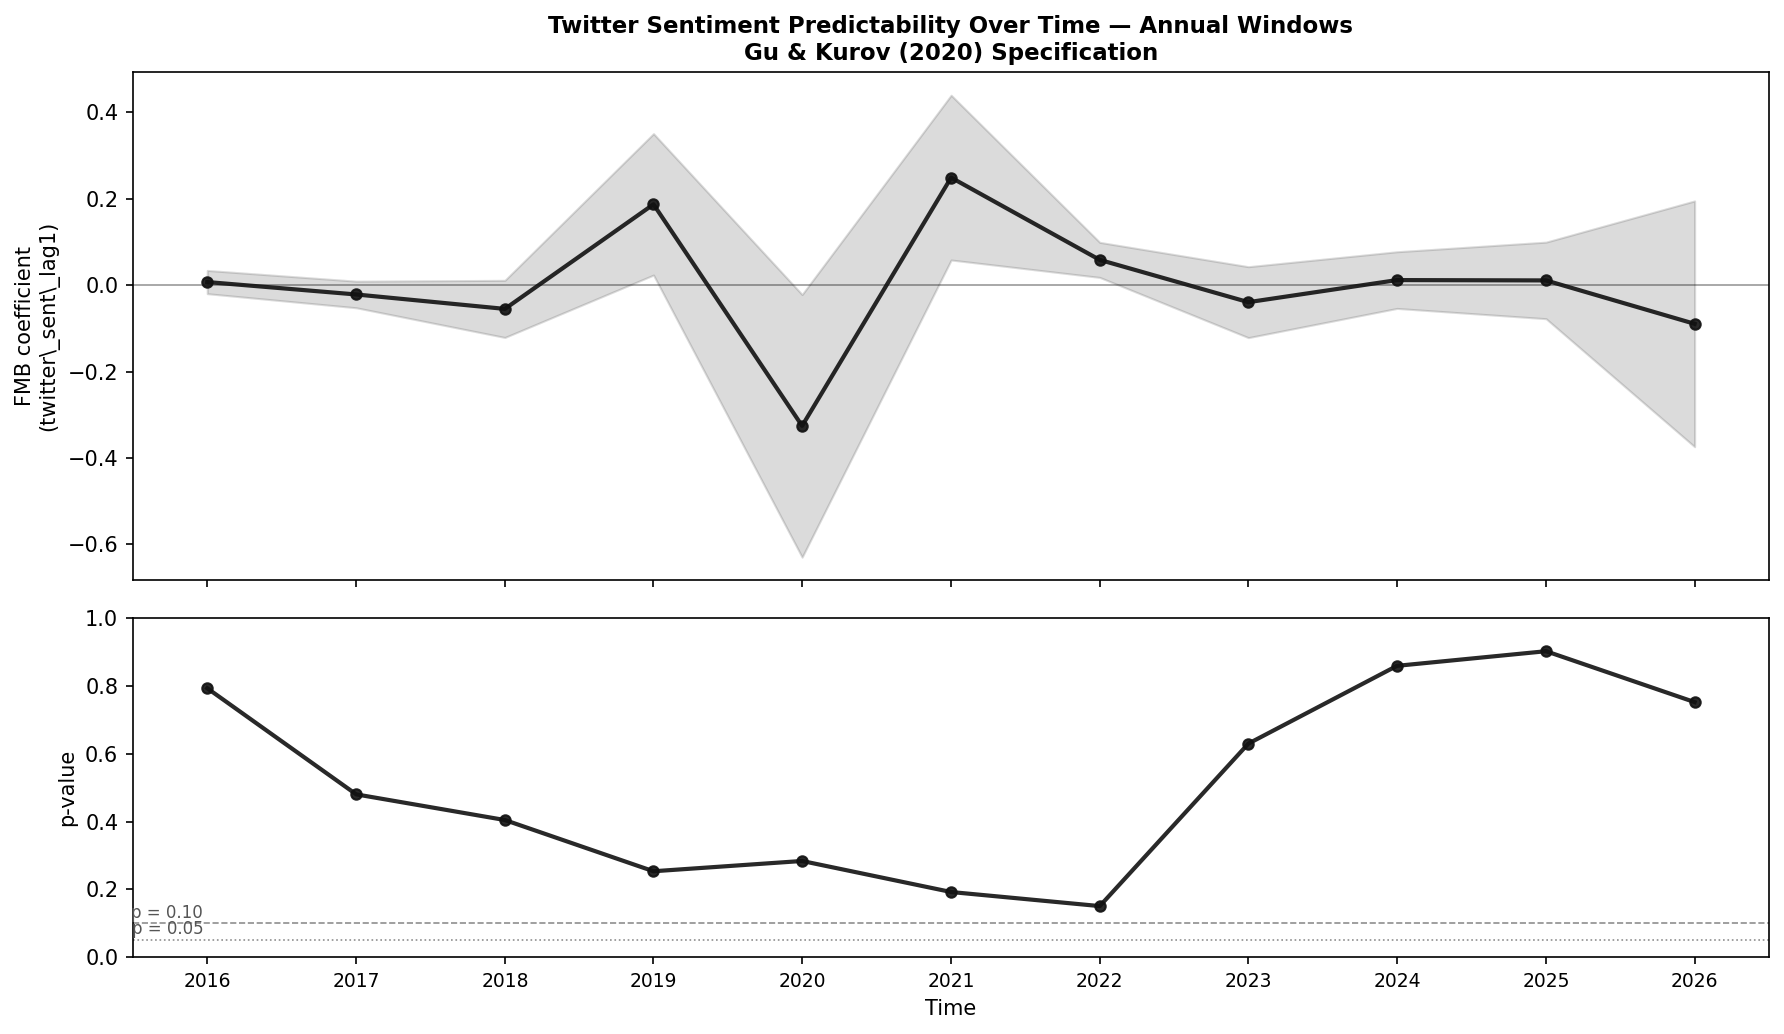
\includegraphics[width=\linewidth]{figures/gk_temporal_annual.png}
\caption{Twitter Sentiment Predictability Over Time --- Annual Windows.
Top panel: Fama-MacBeth coefficient on \texttt{twitter\_sent\_lag1} with $\pm$1 SE band.
Bottom panel: $p$-value; dashed lines at $p = 0.10$ and $p = 0.05$.
Bandwidth = 5 lags; minimum cross-section $N = 30$.}
\label{fig:gk_temporal_annual}
\end{figure}

\begin{figure}[htbp]
\centering
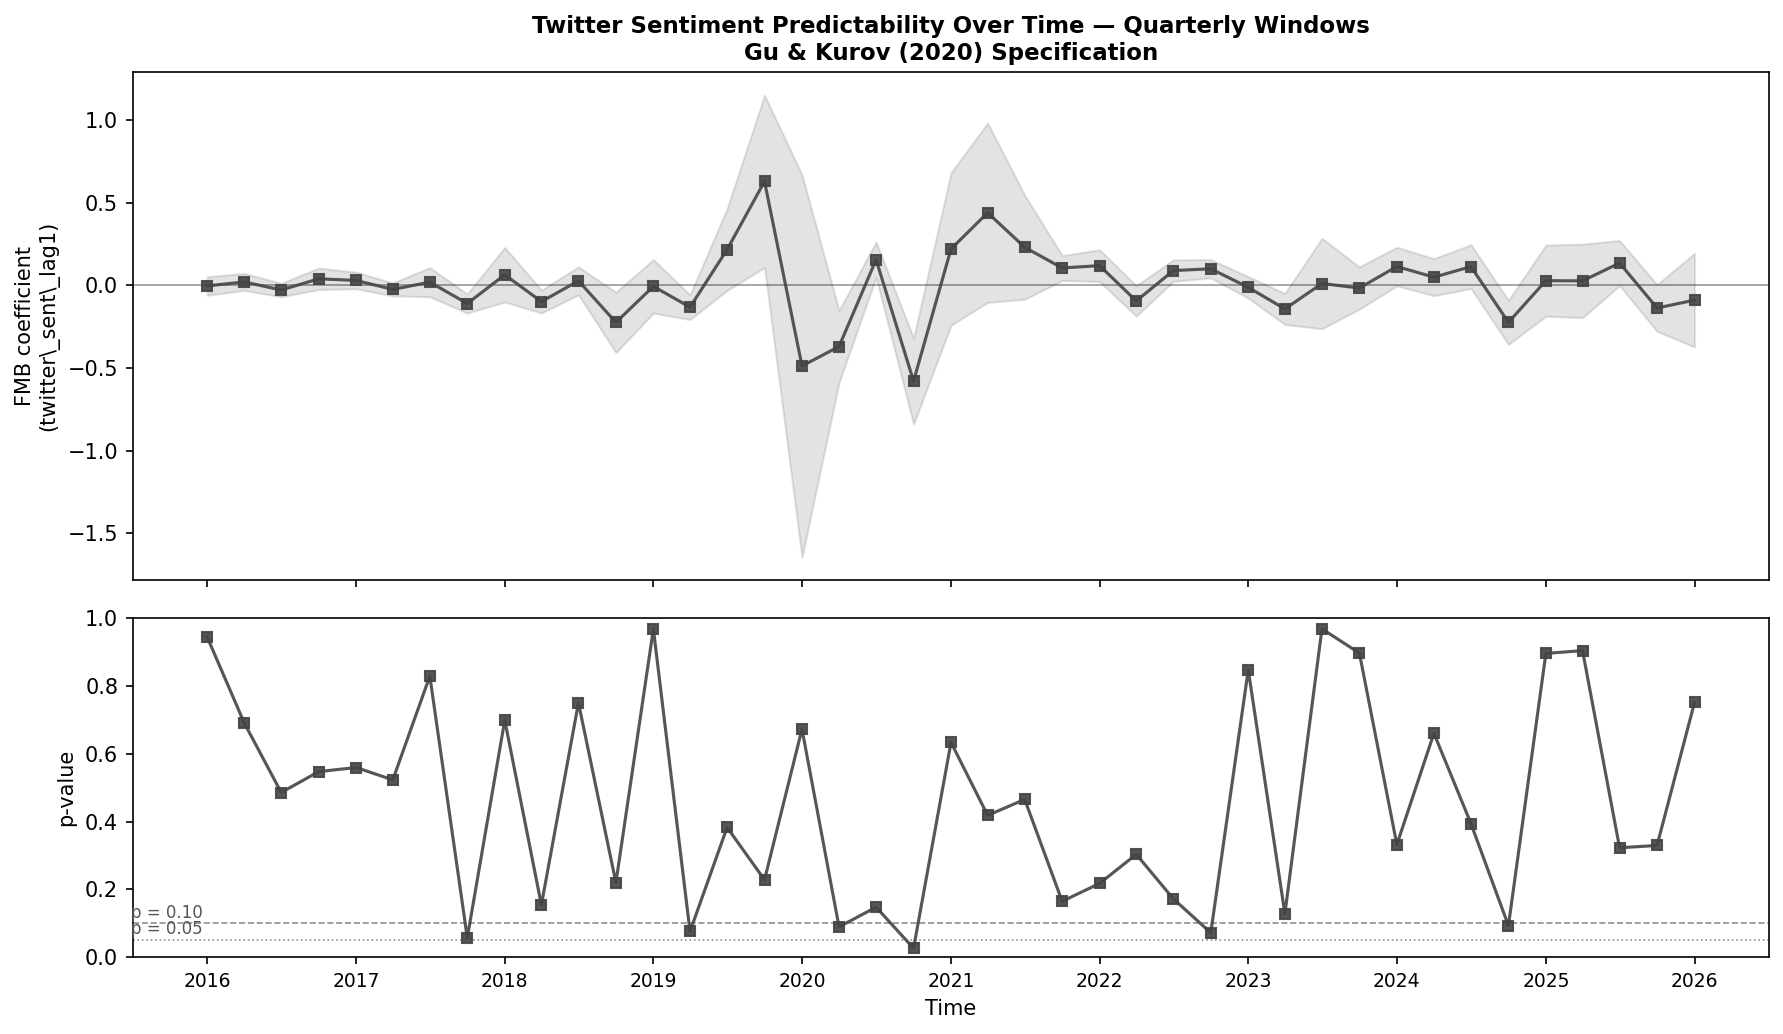
\includegraphics[width=\linewidth]{figures/gk_temporal_quarterly.png}
\caption{Twitter Sentiment Predictability Over Time --- Quarterly Windows.
Top panel: Fama-MacBeth coefficient on \texttt{twitter\_sent\_lag1} with $\pm$1 SE band.
Bottom panel: $p$-value; dashed lines at $p = 0.10$ and $p = 0.05$.
Bandwidth = 4 lags; minimum cross-section $N = 20$.}
\label{fig:gk_temporal_quarterly}
\end{figure}

\begin{figure}[htbp]
\centering
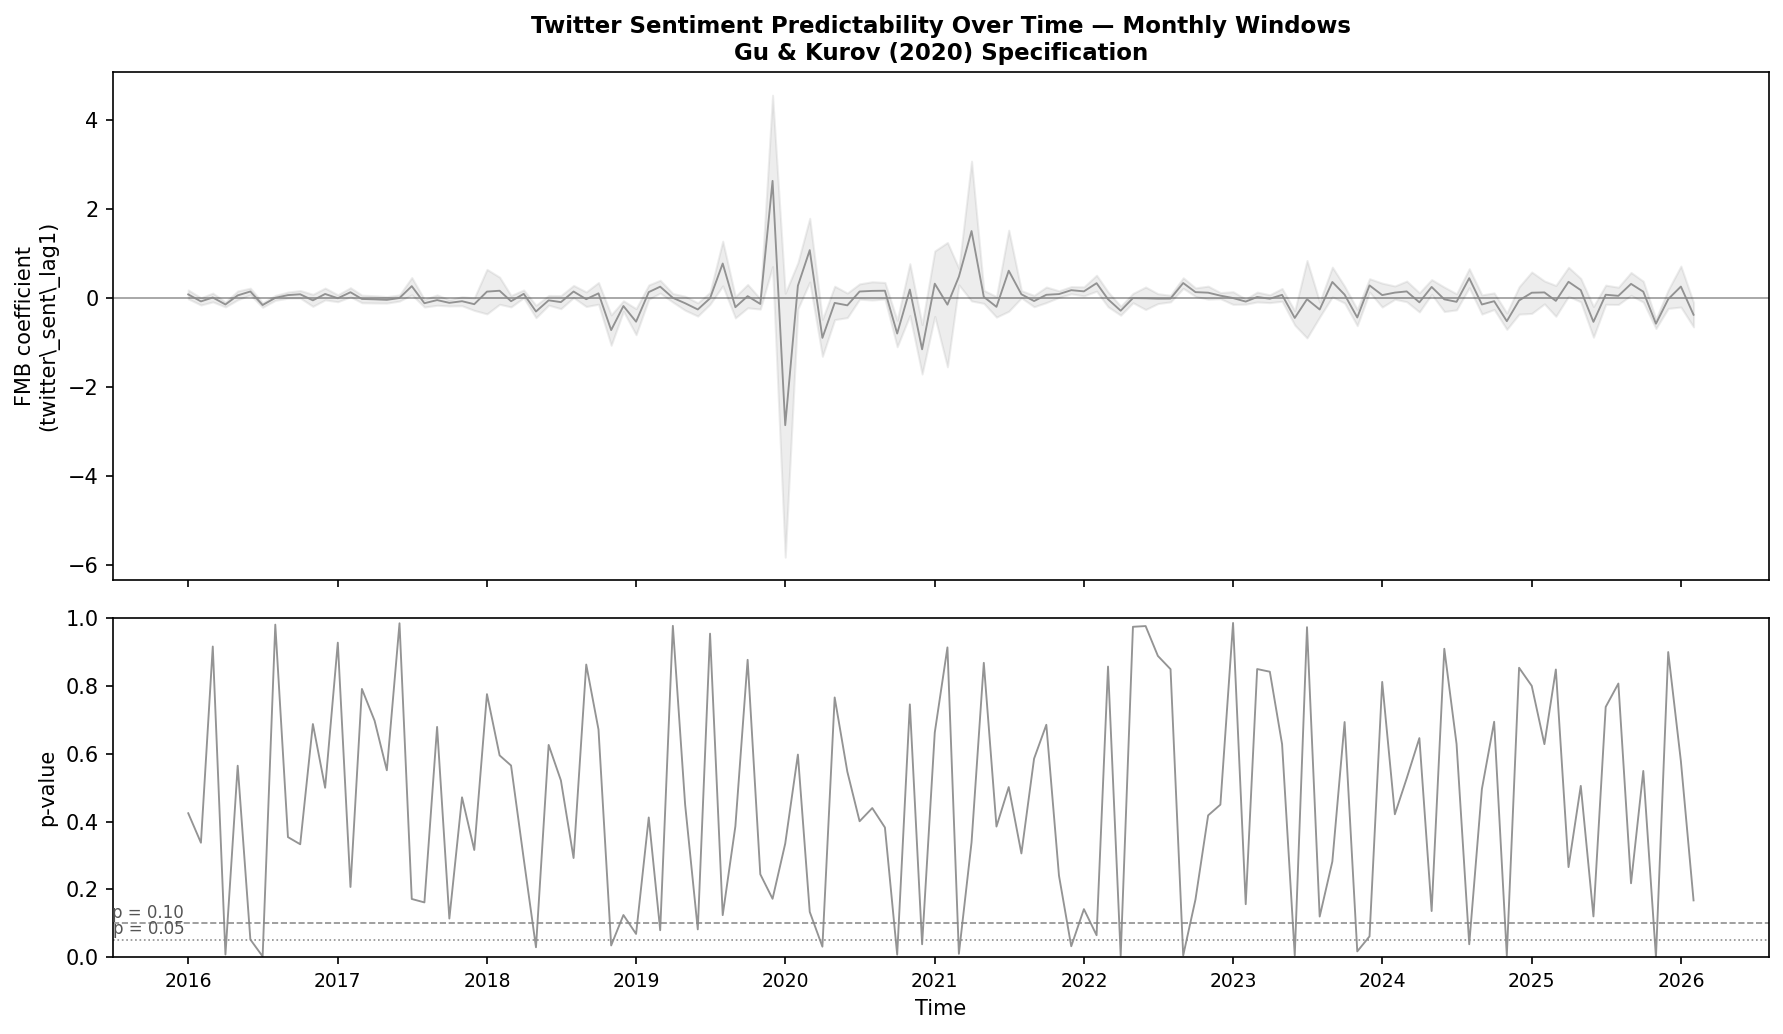
\includegraphics[width=\linewidth]{figures/gk_temporal_monthly.png}
\caption{Twitter Sentiment Predictability Over Time --- Monthly Windows.
Top panel: Fama-MacBeth coefficient on \texttt{twitter\_sent\_lag1} with $\pm$1 SE band.
Bottom panel: $p$-value; dashed lines at $p = 0.10$ and $p = 0.05$.
Bandwidth = 3 lags; minimum cross-section $N = 15$.}
\label{fig:gk_temporal_monthly}
\end{figure}

\medskip

\noindent\textit{Russell 3000 Data Infrastructure --- Completed.}

I updated the data ingestion pipeline (\texttt{clean\_data\_russel.py}) to handle the Bloomberg
export constraints for the Russell 3000. Because the index is too large to export as a single
spreadsheet, each year will arrive as two separate \texttt{.xlsx} files with a consistent naming
convention:
\begin{itemize}
    \item \texttt{bloomberg\_russell\_YYYY\_prices.xlsx} --- \texttt{PX\_OPEN}, \texttt{PX\_CLOSE},
    \texttt{PX\_HIGH}, \texttt{PX\_LOW}, \texttt{PX\_VOLUME}
    \item \texttt{bloomberg\_russell\_YYYY\_sentiment.xlsx} --- bid-ask spread, Twitter/news
    sentiment, RSI, and other non-price fields
\end{itemize}
The script automatically discovers all years present in \texttt{data/raw/}, parses each file
independently, merges the prices and sentiment files on \texttt{(date, ticker)} with an outer
join (so no observations are silently dropped), and concatenates across years into a single
\texttt{russel\_panel.csv}. Overlapping date ranges and accidental field duplication between the
two files are both handled gracefully.

\medskip

\noindent\textit{Paper Drafting --- In Progress.}

Three sections have been drafted and saved to \texttt{output/}:
\begin{itemize}
    \item \textbf{Introduction} (\texttt{draft\_introduction.tex}) --- states the research question,
    motivates the study with the retail trading literature, previews both identification strategies
    and findings including the reverse causality concern, and closes with a roadmap.
    \item \textbf{Literature Review} (\texttt{draft\_literature\_review.tex}) --- covers three threads:
    investor sentiment and asset pricing, social media as an information channel, and causal
    identification in high-frequency panels. Positions the DoubleML contribution relative to Gu \&
    Kurov (2020) and Teti et al.\ (2019).
    \item \textbf{Data} (\texttt{draft\_data.tex}) --- describes the Bloomberg panel, defines all
    variables with their Bloomberg field codes, and documents the three measurement limitations of
    the proprietary sentiment series (opaque classification, temporal aggregation mismatch, and
    selection in coverage).
\end{itemize}
Remaining sections to draft: Methodology, Results, Discussion, Conclusion, Abstract.

\bigskip

\noindent\textbf{Reflection:}

The temporal analysis settles the question of whether the original Gu \& Kurov (2020) effect
existed at some point in the sample and has since decayed. It has not: the predictive coefficient
is flat and insignificant across every year from 2016 to 2025, including the 2016--2017 window
that was the basis for their original finding. The most likely explanations are either that the
Bloomberg composite sentiment measure differs materially from the proprietary dataset used by Gu
\& Kurov, or that the effect was specific to their sample of firms and time period and does not
generalize to the S\&P~500 universe. The long-short strategy results complicate this narrative
slightly --- the strategy earns positive returns in 9 of 10 complete years with Sharpe ratios
occasionally exceeding 1.5 --- but as noted above, this appears to reflect realized cross-sectional
dispersion rather than the sentiment signal driving returns in the direction the regression
predicts.

The data infrastructure work for the Russell 3000 puts a broader robustness check within reach.
Once the Bloomberg exports arrive, running the same FE-OLS and DoubleML specifications on a
universe three times larger will help determine whether the null result is specific to large-cap
S\&P~500 firms or extends to mid- and small-cap stocks where Twitter sentiment might be more
informative relative to institutional coverage.

\bigskip

\noindent\textbf{Questions:}

\begin{enumerate}
    \item The long-short Sharpe ratios vary considerably year to year (from $-$0.05 in 2024 to
    2.04 in 2023) with no obvious macroeconomic explanation. Is this level of cross-year variance
    in a sentiment-sorted strategy expected, or does it suggest a data quality issue in specific
    years of the Bloomberg feed?

    \item Should the Russell 3000 analysis be included as a robustness check in the main paper, or
    treated as a separate extension? Given the drafting timeline, it may be cleaner to reference it
    as in-progress and include a placeholder table.
\end{enumerate}

\end{document}
